\documentclass[float=false, crop=true]{standalone}

\usepackage
{
  amsfonts,
  fp,
  tikz,
}

\usetikzlibrary{automata, positioning, arrows.meta}                             % Tikz macros

\begin{document}

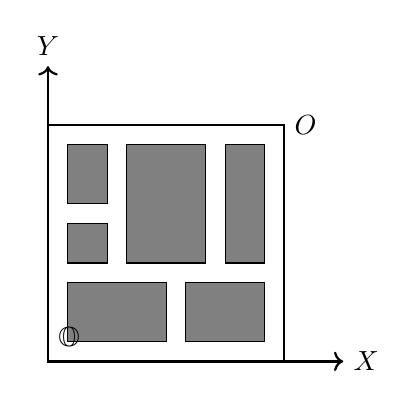
\begin{tikzpicture}[scale=0.25]
\draw [thick, -] (0,0) rectangle (12,12) node[right]{$O$};
\draw[fill=gray] (1,1) rectangle (6,4);
\draw[fill=gray] (11,11) rectangle (9,5);
\draw[fill=gray] (8,11) rectangle (4,5);
\draw[fill=gray] (1,11) rectangle (3,8);
\draw[fill=gray] (1,7) rectangle (3,5);
\draw[fill=gray] (11,1) rectangle (7,4);
\draw [thick,<->] (0,15) node[above]{$Y$}              --
                  (0,0)node[above right]{$\mathbb{O}$} --
                  (15,0) node[right]{$X$};
\end{tikzpicture}

\end{document}
